\documentclass[conference]{IEEEtran}
\IEEEoverridecommandlockouts
% The preceding line is only needed to identify funding in the first footnote. If that is unneeded, please comment it out.
\usepackage{cite}
\usepackage{amsmath,amssymb,amsfonts}
\usepackage{algorithmic}
\usepackage{graphicx}
\usepackage{textcomp}
\usepackage{xcolor}
\usepackage[T1]{fontenc}
\usepackage[numbers,sort&compress]{natbib}
\def\BibTeX{{\rm B\kern-.05em{\sc i\kern-.025em b}\kern-.08em
    T\kern-.1667em\lower.7ex\hbox{E}\kern-.125emX}}
\begin{document}

\title{Enhancing Spatiotemporal Modeling for Egocentric 3D Human Pose Estimation\\
}

\author{\IEEEauthorblockN{Linzhimeng Duan}
\IEEEauthorblockA{\textit{School of Computer Science} \\
\textit{Beijing University of}\\
\textit{Posts and Telecommunications}\\
Beijing, China \\
duanlinzhimeng@bupt.edu.cn}
\and
\IEEEauthorblockN{Jiwei Zhang}
\IEEEauthorblockA{\textit{School of Computer Science} \\
\textit{Beijing University of}\\
\textit{Posts and Telecommunications}\\
Beijing, China \\
jwzhang666@bupt.edu.cn}
\and
\IEEEauthorblockN{Zheyuan Zhang}
\IEEEauthorblockA{\textit{School of Computer Science} \\
\textit{Beijing University of}\\
\textit{Posts and Telecommunications}\\
Beijing, China \\
zzy1998@bupt.edu.cn}
\and
\IEEEauthorblockN{Hong Chen}
\IEEEauthorblockA{\textit{School of Computer Science} \\
\textit{Beijing University of}\\
\textit{Posts and Telecommunications}\\
Beijing, China \\
chenghong76@bupt.edu.cn}
}

\maketitle

\begin{abstract}
Egocentric 3D human pose estimation aims to recover accurate and temporally stable body poses from head-mounted sensors, yet remains challenging due to severe self-occlusion, limited field of view, and rapid motion changes. While recent transformer-based methods model long-range temporal dependencies, they often rely on implicit learning and fail to explicitly enforce anatomical structure and joint-wise temporal consistency inherent in human motion. In this paper, we propose an enhanced spatiotemporal framework that explicitly strengthens both spatial and temporal representations for egocentric 3D pose estimation. Spatially, we incorporate a learnable graph-based module to adaptively model inter-joint relationships guided by skeletal priors. Temporally, we introduce a lightweight joint-wise adaptive temporal smoothing module that enhances local temporal consistency while preserving joint-specific temporal pose patterns. By integrating these components prior to global temporal modeling, our framework provides more coherent spatiotemporal features for subsequent transformer-based reasoning. Extensive experiments on the SELF dataset demonstrate that the proposed method consistently outperforms competitive baselines across multiple evaluation metrics, while incurring only marginal computational overhead and maintaining real-time performance.
\end{abstract}



\begin{IEEEkeywords}
Egocentric 3D Pose Estimation, Spatiotemporal Modeling, Graph Convolution, Transformer
\end{IEEEkeywords}

\section{Introduction}
Egocentric 3D human pose estimation aims to recover full-body 3D poses from head-mounted cameras and sensors, and has recently attracted increasing attention due to its wide applications in virtual reality, augmented reality, and human-computer interaction\citep{b1,b2,b3,b4,b5,b6,b7,b8,b15}. By placing sensors on the wearer, egocentric systems enable unconstrained motion capture without relying on external cameras, offering strong practicality in real-world scenarios~\citep{b1,b2,b4,b5}. However, estimating accurate and temporally stable poses from an egocentric viewpoint remains highly challenging, as large portions of the body are frequently occluded, observations are often incomplete, viewpoints change rapidly with head motion, and pose dynamics can be highly complex\citep{b1,b4,b5,b6,b7}.

To address these challenges, recent studies have increasingly adopted transformer-based architectures to model long-range temporal dependencies in pose sequences. Prior works demonstrate that global temporal attention can effectively capture long-term pose evolution and improve robustness under occlusion and noisy observations~\citep{b1,b2,b8}. Meanwhile, graph-based modeling has been explored to encode anatomical joint relationships and enhance spatial coherence in general 3D human pose estimation~\citep{b9,b10}. Despite their effectiveness, most existing egocentric approaches primarily rely on implicit learning to capture spatial and temporal dependencies, without explicitly enforcing anatomical structure or joint-wise local temporal consistency. This limitation may lead to spatial incoherence and temporal jitter, particularly in challenging egocentric scenarios with rapid motion and severe self-occlusion.

Egocentric 3D human pose sequences, however, exhibit strong structural regularities in both space and time. Spatially, body joints are governed by well-defined anatomical connectivity and kinematic constraints, where explicitly modeling inter-joint relationships can improve spatial consistency~\citep{b9,b10}. Temporally, human pose trajectories are locally smooth, while different joints exhibit distinct temporal characteristics: some joints remain relatively stable, whereas others undergo rapid and irregular pose variations. These observations suggest that explicitly strengthening anatomical joint relations and enforcing joint-wise local temporal consistency can provide a more reliable foundation for subsequent global temporal reasoning.

Motivated by this insight, we build upon a strong transformer-based egocentric pose estimation framework and propose an enhanced spatiotemporal architecture that explicitly reinforces both spatial and temporal representations, while introducing only minimal additional computational overhead. Specifically, we incorporate a Learnable Graph Convolution (LGC) module to integrate skeletal priors with learnable joint dependencies, and a Joint-wise Adaptive Temporal Smoothing (JATS) module to perform lightweight joint-specific local temporal refinement prior to global temporal modeling. Extensive experiments on the SELF dataset demonstrate that the proposed framework consistently outperforms existing methods across multiple evaluation metrics, while maintaining real-time inference efficiency. Comprehensive ablation studies further validate the complementary effects of the proposed spatial and temporal components.

In summary, our main contributions are threefold:
\begin{itemize}
    \item We introduce a Learnable Graph Convolution (LGC) module that explicitly enhances spatial joint relationships by integrating anatomical priors with data-driven graph learning.
    \item We propose a Joint-wise Adaptive Temporal Smoothing (JATS) module that strengthens joint-wise local temporal consistency through lightweight residual refinement.
    \item We achieve competitive performance on egocentric 3D human pose estimation benchmarks with an efficient and unified spatiotemporal framework.
\end{itemize}


\section{Related Work}

\subsection{General 3D Human Pose Estimation}
General 3D human pose estimation aims to recover 3D joint coordinates from monocular or multi-view images and videos, and has been extensively studied. Recent works have increasingly emphasized the explicit modeling of anatomical structure and temporal dynamics. KTPFormer~\cite{b9} introduces kinematic and trajectory priors into a transformer framework, employing graph convolution to enforce skeletal constraints and temporal coherence. MotionAGFormer~\cite{b10} proposes an adaptive graph attention transformer that dynamically learns joint dependencies through multi-scale graph convolutions and temporal attention. TCPFormer~\cite{b11} presents a temporal correlation learning framework using implicit pose proxies to enhance sequence-level temporal modeling.

Other approaches explore alternative architectural designs for efficient structural and temporal reasoning. GraphMLP~\cite{b12} combines graph convolution with multi-layer perceptrons to capture both global and local joint interactions. Cheng et al.~\cite{b13} employ temporal convolutional networks together with a Cylinder Man Model to explicitly handle occlusions and enforce temporal smoothness. PyMAF-X~\cite{b14} extends parametric human mesh recovery by incorporating pyramidal mesh alignment feedback for full-body regression.

While these methods demonstrate the effectiveness of graph-based modeling and temporal reasoning, they are primarily designed for third-person settings and often rely on heavy temporal architectures, which may be suboptimal for egocentric scenarios with strict efficiency constraints.

\subsection{Egocentric 3D Human Pose Estimation}
Egocentric 3D human pose estimation aims to recover full-body poses from head-mounted sensors under severe self-occlusion, limited field of view, and rapid motion changes. FRAME~\cite{b1} leverages geometric representations together with transformer-based temporal modeling to achieve real-time egocentric pose estimation. REWIND~\cite{b2} introduces cascaded diffusion-based denoising with identity-conditioned refinement to improve pose fidelity and temporal stability. Wang et al.~\cite{b3} further enhance egocentric pose estimation by incorporating motion refinement strategies to stabilize pose sequences captured by head-mounted cameras. Dai et al.~\cite{b4} present the SLOPER4D dataset and a large-scale egocentric pose estimation framework, while Wang et al.~\cite{b5} employ spatio-temporal optimization with learned motion priors to reduce temporal jitter. Akada et al.~\cite{b6,b7} propose egocentric datasets and transformer-based architectures that exploit depth and temporal cues to address self-occlusion, and EgoPoseFormer~\cite{b8} presents a two-stage transformer framework with pose proposals and deformable attention for egocentric pose refinement.

Despite the progress achieved by these methods, most existing approaches primarily focus on global temporal modeling or sequence-level refinement, while explicit modeling of anatomical structure and joint-wise local temporal consistency remains limited. In contrast, our work explicitly strengthens spatial anatomical relations and joint-adaptive local temporal consistency as lightweight inductive biases prior to global temporal modeling, providing a complementary and efficient enhancement for egocentric 3D human pose estimation.




\begin{figure*}[htbp]
\centerline{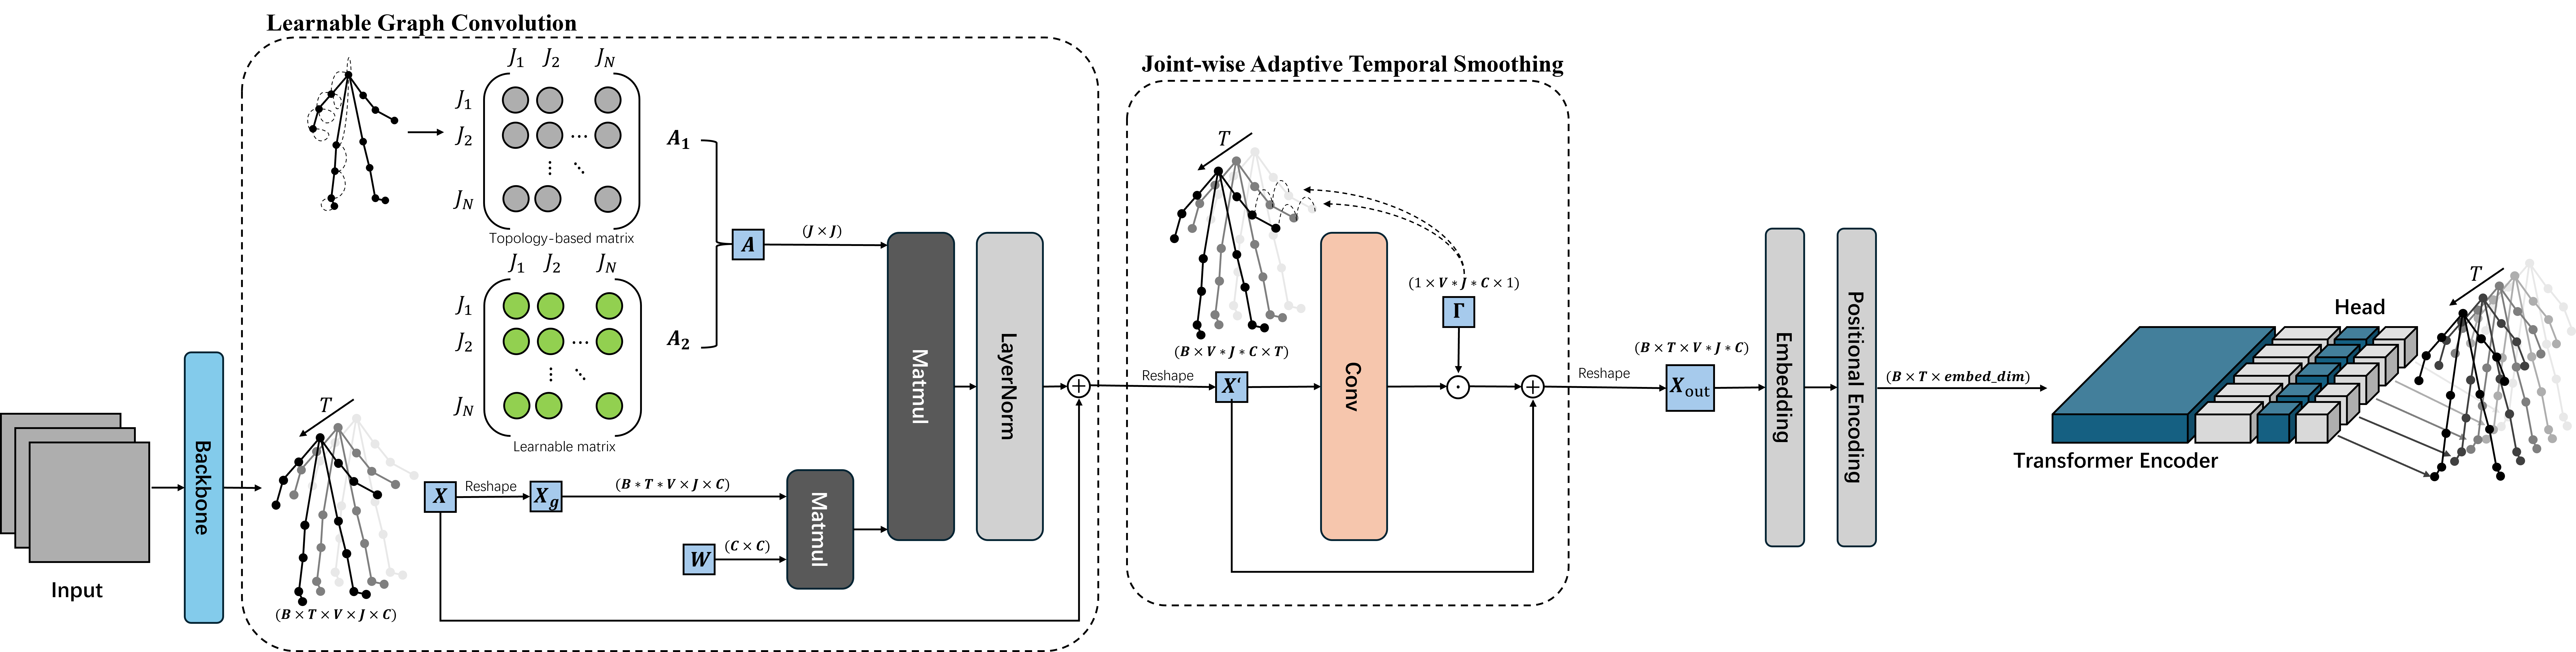
\includegraphics[width=1\textwidth]{fig1.png}}
\caption{Overview of the proposed model architecture. The pose estimates produced by the backbone network are first processed by the Learnable Graph Convolution (LGC) module to explicitly enhance spatial joint relationships. The resulting features are then fed into the Joint-wise Adaptive Temporal Smoothing (JATS) module, which performs lightweight, joint-level local temporal smoothing to stabilize pose trajectories and improve short-term temporal consistency. The refined features are subsequently passed to the temporal Transformer for global temporal reasoning, producing the final pose sequence.}
\label{fig}
\end{figure*}

\section{Method}
Our approach is built upon the FRAME~\cite{b1} architecture. We retain its backbone network for feature extraction and 3D joint coordinate regression, as well as the original Transformer encoder for global temporal modeling. To explicitly enhance spatial structure and local temporal consistency prior to transformer-based reasoning, we insert two lightweight modules before the Transformer encoder: a Learnable Graph Convolution (LGC) module for spatial refinement, followed by a Joint-wise Adaptive Temporal Smoothing (JATS) module for local temporal enhancement.












\subsection{Learnable Graph Convolution}\label{AA}
To explicitly model structured spatial relationships among human body joints, we introduce a Learnable Graph Convolution (LGC) module as a spatial refinement stage prior to temporal modeling. The LGC module enhances joint representations by incorporating anatomical priors while allowing flexible, data-driven modeling of inter-joint dependencies. Through a lightweight residual design, it strengthens spatial coherence without altering the original 3D coordinate representation or introducing significant computational overhead.

Given input joint features $\mathbf{X} \in \mathbb{R}^{B \times T \times V \times J \times 3}$, where $B$ denotes the batch size, $T$ the temporal length, $V$ the number of views, and $J$ the number of joints, the input is reshaped into a graph-compatible representation $\mathbf{X}_g \in \mathbb{R}^{(B \cdot T \cdot V) \times J \times 3}$. The core of the LGC module is a hybrid adjacency matrix that combines fixed anatomical connectivity and a learnable joint relationship matrix. Specifically, a fixed adjacency matrix $\mathbf{A}_1 \in \mathbb{R}^{J \times J}$ is constructed based on the human skeletal kinematic tree, including self-loops and physically connected joint pairs, while a learnable adjacency matrix $\mathbf{A}_2 \in \mathbb{R}^{J \times J}$ is initialized uniformly and optimized during training. The final adjacency matrix is obtained via a learnable convex combination,
\begin{equation}
\tilde{\mathbf{A}} = (1 - \sigma(\alpha)) \mathbf{A}_1 + \sigma(\alpha) \mathbf{A}_2,
\end{equation}
where $\alpha$ is a learnable scalar and $\sigma(\cdot)$ denotes the sigmoid function. After normalization, graph convolution is performed as
\begin{equation}
\mathbf{Y} = \mathbf{A} \mathbf{X}_g \mathbf{W},
\end{equation}
where $\mathbf{W}$ is a learnable weight matrix. In this work, a single graph convolution layer is employed for spatial refinement. The output is reshaped back to $\mathbb{R}^{B \times T \times V \times J \times 3}$ and integrated via a residual formulation,
\begin{equation}
\mathbf{X}_{\text{enhanced}} = \mathbf{X}_{\text{in}} + \lambda \cdot \text{LayerNorm}(\mathbf{Y}),
\end{equation}
where $\lambda$ is a learnable scalar, and LayerNorm is applied along the coordinate dimension. The enhanced features are then passed to the proposed JATS module, providing a spatially coherent foundation for subsequent temporal modeling.











\begin{table*}[htbp]
\caption{Comparison with representative and recent egocentric 3D human pose estimation methods. The proposed approach achieves improved accuracy across multiple evaluation metrics while maintaining comparable inference efficiency.}
\begin{center}
\begin{tabular}{c c c c c}
\hline
{Method}& {\textit{Inference(ms,$\downarrow$)}}& {\textit{MPJPE(mm,$\downarrow$)}}& {\textit{PA-MPJPE(mm,$\downarrow$)}}& {\textit{3D-PCK(\%,$\uparrow$)}}\\
\hline 
{EgoPW\cite{b5}} & {\textit{6.91}}& {\textit{125.63}}& {\textit{76.55}}& {\textit{60.84}} \\
{Egoglass\cite{b15}} & {\textit{8.52}}& {\textit{122.33}}& {\textit{72.05}}& {\textit{63.20}} \\
{UnrealEgo\cite{b6}} & {\textit{7.42}}& {\textit{112.46}}& {\textit{69.87}}& {\textit{59.31}} \\
{EgoPoseFormer\cite{b8}} & {\textit{13.32}}& {\textit{70.15}}& {\textit{43.96}}& {\textit{75.05}} \\
{EgoWholeMocap\cite{b3}} & {\textit{15.25}}& {\textit{66.82}}& {\textit{38.16}}& {\textit{79.63}} \\
{FRAME\cite{b1}} & \textbf{\textit{2.51}}& {\textit{48.28}}& {\textit{36.80}}& {\textit{92.80}} \\
\textbf{Ours} & \textit{2.60}& \textbf{\textit{47.75}}& \textbf{\textit{35.58}}& \textbf{\textit{92.94}} \\
\hline
\end{tabular}
\label{tab1}
\end{center}
\end{table*}












\subsection{Joint-wise Adaptive Temporal Smoothing}
To enhance temporal consistency while preserving joint-specific temporal characteristics, we introduce a Joint-wise Adaptive Temporal Smoothing (JATS) module prior to the Transformer encoder. Unlike heavy temporal modeling strategies, JATS explicitly enforces short-term temporal coherence through lightweight, joint-adaptive local refinement, serving as an effective pre-processing stage before global temporal attention.


Given a 3D joint sequence $\mathbf{X} \in \mathbb{R}^{B \times T \times V \times J \times 3}$, the input is first rearranged along the temporal dimension and reshaped into a channel-first representation $\mathbf{X}' \in \mathbb{R}^{B \times C \times T}$, where $C = V \cdot J \cdot 3$. A depth-wise temporal convolution is then applied along the temporal axis, such that each joint-coordinate channel is processed independently, enabling efficient local temporal filtering without cross-joint interference. To adaptively control the smoothing strength for different joints and coordinates, a learnable joint-wise and coordinate-aware gating mechanism is introduced, and the refined features are combined with the original input via a residual formulation,
\begin{equation}
\mathbf{X}_{\text{out}} = \mathbf{X}' + \Gamma \odot \text{Conv}(\mathbf{X}'),
\end{equation}
where $\Gamma \in \mathbb{R}^{1 \times C \times 1}$ denotes learnable gates and $\odot$ represents element-wise multiplication. This design allows more stable joints to benefit from stronger smoothing while preserving high-frequency variations for highly dynamic joints. Finally, the gated features are reshaped back to the original spatiotemporal format and fed into the embedding layer and Transformer encoder. The proposed JATS module introduces minimal computational overhead while providing an explicit inductive bias for modeling heterogeneous joint dynamics.

Each gate corresponds to a specific joint-coordinate channel, allowing the model to adaptively balance between raw joint trajectories and temporally smoothed signals. More stable joints tend to benefit from stronger smoothing, while highly dynamic joints preserve higher-frequency motion patterns. This adaptive mechanism is fully differentiable and optimized end-to-end with the overall network.

Finally, the gated features are reshaped back to the original spatiotemporal format and fed into the embedding layer and Transformer encoder for global temporal reasoning. The proposed JATS module introduces minimal computational overhead, yet provides an effective inductive bias for modeling heterogeneous joint dynamics, complementing the long-range temporal modeling capability of the Transformer.





\section{Experiments}
\subsection{Dataset}
The SELF dataset~\cite{b1} is a large-scale benchmark for egocentric 3D human pose estimation, capturing multimodal data from 14 subjects. Each subject performs two recording sessions with varied clothing to enhance visual diversity. Each session begins with a short calibration stage, followed by 50 scripted actions (e.g., sports and daily activities), each lasting approximately 20 seconds with short pauses in between, covering a wide range of motion patterns. During recording, participants interact naturally with their surroundings while wearing VR headsets equipped with forward-facing cameras.

The dataset provides stereo egocentric videos, 6D device poses, markerless full-body motion capture, and synchronized multi-view recordings from a 120-camera studio, totaling over 7 hours of data (approximately 1.6 million images). A separate test set containing two additional subjects is provided for unbiased evaluation, contributing around 1 hour of data. For each frame, the dataset includes dual fisheye images $I_t \in \mathbb{R}^{2 \times 3 \times H \times W}$, floor-aligned device poses $T_D(t) \in SE(3)$, and ground-truth 3D joint positions $J_t \in \mathbb{R}^{J \times 3}$. These rich annotations enable reliable training and evaluation for egocentric 3D pose estimation.


\subsection{Metrics}
Following prior works, we evaluate all methods using the mean per-joint position error (MPJPE) in millimeters. In addition, we report Procrustes-aligned MPJPE (PA-MPJPE) to assess structural alignment accuracy, and the 3D percentage of correct keypoints (3D-PCK) measured within a 10 cm distance threshold. These metrics are widely adopted in egocentric pose estimation benchmarks and reflect both positional accuracy and structural consistency, which are closely related to temporal stability in sequential predictions.


\subsection{Implementation Details}
All models are trained using the AdamW optimizer with a batch size of 16. During training, an $\ell_2$ loss is applied to supervise the predicted 3D joint coordinates. We adopt a two-stage training strategy following prior work. In the first stage, the network is optimized in camera coordinates. In the second stage, the temporal Transformer module is further trained using global (world) coordinates to enhance temporal consistency and global pose accuracy. The learning rate for the Transformer is set to $3 \times 10^{-4}$, and training is conducted for 4 epochs.


\subsection{Comparison}
We compare the proposed method with multiple representative egocentric 3D human pose estimation approaches, including the baseline FRAME~\cite{b1} and several prior works, under the same evaluation protocol. All methods are evaluated locally using their officially released pretrained models in a unified testing environment to ensure a fair comparison.

As shown in Table~\ref{tab1}, the proposed method consistently achieves superior or competitive accuracy compared with existing approaches. In particular, our method demonstrates clear improvements over the baseline and prior methods, indicating more accurate and temporally stable 3D pose estimation under challenging egocentric conditions. These results suggest that explicitly strengthening spatial joint relationships and joint-aware local temporal modeling effectively enhances pose estimation performance.

In terms of efficiency, the proposed framework maintains inference latency comparable to the baseline model, incurring only marginal additional computational overhead. Despite introducing extra spatial and temporal refinement modules, the overall runtime remains within the real-time range, demonstrating that the proposed design is lightweight and practical for deployment.

Overall, the comparison results show that the proposed method achieves a favorable balance between accuracy and efficiency, providing a practical improvement over existing egocentric 3D human pose estimation approaches without sacrificing real-time performance.



\subsection{Ablation Study}
\begin{table}[htbp]
\caption{Ablation study of the proposed spatial and temporal modules. We report MPJPE, PA-MPJPE, and 3D-PCK for the baseline FRAME~\cite{b1} model, the model with Learnable Graph Convolution (LGC), and the full model with both LGC and Joint-wise Adaptive Temporal Smoothing (JATS).}
\begin{center}
\begin{tabular}{c c c c}
\hline
{Method}& {\textit{MPJPE(mm,$\downarrow$)}}& {\textit{PA-MPJPE(mm,$\downarrow$)}}& {\textit{3D-PCK(\%,$\uparrow$)}}\\
\hline 
{Baseline} & {48.28} & {36.80} & {92.80} \\
{LGC} & {47.84} & {35.63} & \textbf{92.98} \\
{LGC+JATS (Ours)} & \textbf{47.75} & \textbf{35.58} & {92.94} \\
\hline
\end{tabular}
\label{tab2}
\end{center}
\end{table}


As shown in Table~\ref{tab2}, introducing the Learnable Graph Convolution (LGC) module consistently improves performance over the baseline model. By explicitly modeling anatomical joint relationships, LGC enhances spatial coherence among body joints, leading to reduced MPJPE and PA-MPJPE, as well as improved 3D-PCK. These results demonstrate the effectiveness of strengthening spatial structure through structured joint interactions in egocentric pose estimation.

Further incorporating the proposed Joint-wise Adaptive Temporal Smoothing (JATS) module yields additional performance gains. The improvement indicates that enforcing joint-adaptive local temporal consistency prior to global temporal modeling helps stabilize pose trajectories and complements the spatial refinement provided by LGC. Together, the two modules form a unified spatiotemporal enhancement that improves both accuracy and temporal coherence.


\subsection{Hyperparameter Analysis}

\begin{table}[htbp]
\caption{Comparison of different temporal kernel sizes used in the Joint-wise Adaptive Temporal Smoothing (JATS) module.}
\begin{center}
\begin{tabular}{c c c c}
\hline
{Kernel Size}& {\textit{MPJPE(mm,$\downarrow$)}}& {\textit{PA-MPJPE(mm,$\downarrow$)}}& {\textit{3D-PCK(\%,$\uparrow$)}}\\
\hline
{1} & {48.50} & {35.93} & {92.79} \\
{2} & {48.31} & {35.94} & {92.72} \\
{3} & \textbf{47.75} & \textbf{35.58} & \textbf{92.94} \\
{4} & {49.78} & {37.33} & {92.20} \\
{5} & {48.69} & {35.66} & {92.86} \\
\hline
\end{tabular}
\label{tab_hyper}
\end{center}
\end{table}

As shown in Table~\ref{tab_hyper}, we compare different temporal kernel sizes for the proposed Joint-wise Adaptive Temporal Smoothing (JATS) module in order to identify the most effective hyperparameter setting. A kernel size of 1, which does not incorporate temporal context, leads to inferior performance due to the lack of local temporal refinement. Increasing the kernel size to 3 consistently improves all evaluation metrics, indicating that incorporating short-range temporal context is beneficial for stabilizing joint trajectories. Further increasing the kernel size to 5 does not yield additional improvements and slightly degrades performance. Based on these results, a kernel size of 3 is adopted in all experiments as it provides the best overall accuracy while maintaining a lightweight temporal design.






\section{Conclusion}
In this paper, we propose a lightweight spatiotemporal enhancement framework for egocentric 3D human pose estimation. Built upon the FRAME architecture, our method explicitly strengthens spatial structure and local temporal consistency prior to transformer-based global temporal modeling. Specifically, we introduce a Learnable Graph Convolution module that integrates anatomical priors with data-driven graph learning to refine spatial joint relationships while preserving precise 3D coordinates, and a Joint-wise Adaptive Temporal Smoothing module that performs joint-level local temporal refinement to stabilize pose sequences. Extensive experiments and ablation studies demonstrate that both components contribute consistently to performance improvements and that their combination yields complementary benefits. Importantly, the proposed enhancements introduce only marginal computational overhead, maintaining real-time inference performance. Overall, this work highlights the effectiveness of explicitly reinforcing spatial and local temporal modeling as a practical extension to transformer-based frameworks for egocentric 3D human pose estimation.










\begin{thebibliography}{00}
\bibitem{b1} Camiletto A B, Wang J, Alvarado E, et al. FRAME: Floor-aligned Representation for Avatar Motion from Egocentric Video[C]//Proceedings of the Computer Vision and Pattern Recognition Conference. 2025: 17497-17507.
\bibitem{b2} Lee J, Xu W, Richard A, et al. REWIND: Real-Time Egocentric Whole-Body Motion Diffusion with Exemplar-Based Identity Conditioning[C]//Proceedings of the Computer Vision and Pattern Recognition Conference. 2025: 7095-7104.
\bibitem{b3} Wang J, Cao Z, Luvizon D, et al. Egocentric whole-body motion capture with fisheyevit and diffusion-based motion refinement[C]//Proceedings of the IEEE/CVF Conference on Computer Vision and Pattern Recognition. 2024: 777-787.
\bibitem{b4} Wang J, Luvizon D, Xu W, et al. Scene-aware egocentric 3d human pose estimation[C]//Proceedings of the IEEE/CVF Conference on Computer Vision and Pattern Recognition. 2023: 13031-13040.
\bibitem{b5} Wang J, Liu L, Xu W, et al. Estimating egocentric 3d human pose in global space[C]//Proceedings of the IEEE/CVF International Conference on Computer Vision. 2021: 11500-11509.
\bibitem{b6} Akada H, Wang J, Shimada S, et al. Unrealego: A new dataset for robust egocentric 3d human motion capture[C]//European Conference on Computer Vision. Cham: Springer Nature Switzerland, 2022: 1-17.
\bibitem{b7} Akada H, Wang J, Golyanik V, et al. 3d human pose perception from egocentric stereo videos[C]//Proceedings of the IEEE/CVF Conference on computer vision and pattern recognition. 2024: 767-776.
\bibitem{b8} Yang C, Tkach A, Hampali S, et al. Egoposeformer: A simple baseline for egocentric 3d human pose estimation[J]. arXiv preprint arXiv:2403.18080, 2024, 1(2): 6.
\bibitem{b9} Peng J, Zhou Y, Mok P Y. Ktpformer: Kinematics and trajectory prior knowledge-enhanced transformer for 3d human pose estimation[C]//Proceedings of the IEEE/CVF Conference on Computer Vision and Pattern Recognition. 2024: 1123-1132.
\bibitem{b10} Mehraban S, Adeli V, Taati B. Motionagformer: Enhancing 3d human pose estimation with a transformer-gcnformer network[C]//Proceedings of the IEEE/CVF winter conference on applications of computer vision. 2024: 6920-6930.
\bibitem{b11} Liu J, Liu M, Liu H, et al. Tcpformer: Learning temporal correlation with implicit pose proxy for 3d human pose estimation[C]//Proceedings of the AAAI Conference on Artificial Intelligence. 2025, 39(5): 5478-5486.
\bibitem{b12} Li W, Liu M, Liu H, et al. GraphMLP: A graph MLP-like architecture for 3D human pose estimation[J]. Pattern Recognition, 2025, 158: 110925.
\bibitem{b13} Cheng Y, Yang B, Wang B, et al. Occlusion-aware networks for 3d human pose estimation in video[C]//Proceedings of the IEEE/CVF international conference on computer vision. 2019: 723-732.
\bibitem{b14} Zhang H, Tian Y, Zhang Y, et al. Pymaf-x: Towards well-aligned full-body model regression from monocular images[J]. IEEE Transactions on Pattern Analysis and Machine Intelligence, 2023, 45(10): 12287-12303.
\bibitem{b15} D. Zhao, Z. Wei, J. Mahmud, and J.-M. Frahm, “EgoGlass: Egocentric-View Human Pose Estimation From an Eyeglass Frame,” in 2021 International Conference on 3D Vision (3DV), Feb. 2021, pp. 32–41. doi: 10.1109/3DV53792.2021.00014.

\end{thebibliography}
\end{document}
